%\VignetteEngine{knitr::knitr}
%\VignetteIndexEntry{Flexible Logo plots of symbols and alphanumeric strings using Logolas}
%\VignettePackage{Logolas}

% To compile this document
% library('knitr'); rm(list=ls()); knit('Logolas/vignettes/logolas.Rnw')
% library('knitr'); rm(list=ls()); knit2pdf('Logolas/vignettes/logolas.Rnw'); openPDF('logolas.pdf')
% !Rnw weave = knitr

\documentclass[12pt]{article}\usepackage[]{graphicx}\usepackage[usenames,dvipsnames]{color}
%% maxwidth is the original width if it is less than linewidth
%% otherwise use linewidth (to make sure the graphics do not exceed the margin)
\makeatletter
\def\maxwidth{ %
  \ifdim\Gin@nat@width>\linewidth
    \linewidth
  \else
    \Gin@nat@width
  \fi
}
\makeatother

\definecolor{fgcolor}{rgb}{0.345, 0.345, 0.345}
\newcommand{\hlnum}[1]{\textcolor[rgb]{0.686,0.059,0.569}{#1}}%
\newcommand{\hlstr}[1]{\textcolor[rgb]{0.192,0.494,0.8}{#1}}%
\newcommand{\hlcom}[1]{\textcolor[rgb]{0.678,0.584,0.686}{\textit{#1}}}%
\newcommand{\hlopt}[1]{\textcolor[rgb]{0,0,0}{#1}}%
\newcommand{\hlstd}[1]{\textcolor[rgb]{0.345,0.345,0.345}{#1}}%
\newcommand{\hlkwa}[1]{\textcolor[rgb]{0.161,0.373,0.58}{\textbf{#1}}}%
\newcommand{\hlkwb}[1]{\textcolor[rgb]{0.69,0.353,0.396}{#1}}%
\newcommand{\hlkwc}[1]{\textcolor[rgb]{0.333,0.667,0.333}{#1}}%
\newcommand{\hlkwd}[1]{\textcolor[rgb]{0.737,0.353,0.396}{\textbf{#1}}}%
\let\hlipl\hlkwb

\usepackage{framed}
\makeatletter
\newenvironment{kframe}{%
 \def\at@end@of@kframe{}%
 \ifinner\ifhmode%
  \def\at@end@of@kframe{\end{minipage}}%
  \begin{minipage}{\columnwidth}%
 \fi\fi%
 \def\FrameCommand##1{\hskip\@totalleftmargin \hskip-\fboxsep
 \colorbox{shadecolor}{##1}\hskip-\fboxsep
     % There is no \\@totalrightmargin, so:
     \hskip-\linewidth \hskip-\@totalleftmargin \hskip\columnwidth}%
 \MakeFramed {\advance\hsize-\width
   \@totalleftmargin\z@ \linewidth\hsize
   \@setminipage}}%
 {\par\unskip\endMakeFramed%
 \at@end@of@kframe}
\makeatother

\definecolor{shadecolor}{rgb}{.97, .97, .97}
\definecolor{messagecolor}{rgb}{0, 0, 0}
\definecolor{warningcolor}{rgb}{1, 0, 1}
\definecolor{errorcolor}{rgb}{1, 0, 0}
\newenvironment{knitrout}{}{} % an empty environment to be redefined in TeX

\usepackage{alltt}

\newcommand{\Logolas}{\textit{Logolas}}
\usepackage{dsfont}
\usepackage{cite}



\RequirePackage{/Library/Frameworks/R.framework/Versions/3.3/Resources/library/BiocStyle/resources/tex/Bioconductor}

\AtBeginDocument{\bibliographystyle{/Library/Frameworks/R.framework/Versions/3.3/Resources/library/BiocStyle/resources/tex/unsrturl}}



\author{Kushal K Dey, Dongyue Xie, Matthew Stephens  \\[1em]
\small{Dept. of Statistics, The University of Chicago} \mbox{ }\\
\small{\texttt{$^*$Correspondending Email: kkdey@uchicago.edu}}}


\bioctitle[ Flexible Logo plots of symbols and alphanumeric strings using \Logolas{}]{Flexible Logo plots of symbols and alphanumeric strings using \Logolas{}}
\IfFileExists{upquote.sty}{\usepackage{upquote}}{}
\begin{document}

\maketitle

\begin{abstract}
\vspace{1em}
Logo plots are popular in genomic studies for sequence alignment and motif detection. However, logo plots have been restrictive in its scope due to limited size of the library of symbols used by logo plotting tools and packages  and the lack of flexibility in extending it to other applications. In this package, we provide an easy and flexible interface for the user to plot logos. More importantly, we extend the library of logos from A, C, T, G (library of symbols in seqLogo) and English alphabets (library of symbols in RWebLogo, motifStack) to include numbers and alpha-numeric strings with provision for punctuations and arrows. It also provides the user with a simple graphical interface to create her own logo and add to her personal library.
In this vignette, we discuss a number of applications in genomics and beyond where such flexible logo plots can be effective in visualizing patterns.

\vspace{1em}
\textbf{\Logolas{} version:} 1.2.1 \footnote{This document used the vignette from \Bioconductor{} package \Biocpkg{CountClust, DESeq2} as \CRANpkg{knitr} template}
\end{abstract}



\newpage

\tableofcontents

\section{Introduction}

Ever since its introduction due to Schneider and Stephens (1990), sequence logos have proved to be an effective tool in informative visualization of patterns in aligned sets of sequences. There are several existing packages for plotting sequence logos, like \textit{seqLogo}, \textit{seq2Logo}, \textit{motifStack} etc.

We introduce another Logo visualization package called \textit{Logolas} which addresses some limitations of the above packages and makes logo visualization a more generic tool with potential applications in a much wider scope of problems, in comparison to the existing softwares. Some features of \textit{Logolas} are as follows.

- \textbf{EDLogo Representation} : General logo plotting softwares highlight only enrichment of certain symbols, but Logolas allows the user to highlight both enrichment and depletion of symbols at any position, leading to more parsimonious and visually appealing representation.

- \textbf{Strings as symbols} : General logo building softwares have limited library of symbols usually restricted to English alphabets. Logolas allows the user to plot symbols for any alphanumeric string, comprising of English alphabets, numbers, punctuation marks, arrows etc. It also provides an easy interface for the user to create her own logo and add to the library of symbols that can be plotted (check the Vignette).


- \textbf{Dirichlet Adaptive Shrinkage} : Most existing logo plotting tools take position weight matrix (PWM) as input for the logo plot and do not adapt well to the scale of the underlying positional frequencies from which the PWM is created. In Logolas, we provide a Dirichlet Adaptive Shrinkage method (dash) approach for adaptively scaling the heights of the logos based on the frequency scale. This approach is similar in lines to the **ashr** software due to M. Stephens (2016).


- \textbf{Better stylizations} : Logolas also allows for new and flexible stylizations of the logos, involving color palettes, new fill and border styles, several options for determining heights of the logos etc. We also show how to plot multi-panel Logolas plots and combine Logolas plots with ggplot2 graphics.


\newpage

\section{\Logolas{} Installation}

\Logolas{} loads as dependencies the following CRAN-R package : \CRANpkg{grid}, \CRANpkg{gridExtra}, \CRANpkg{graphics}, \CRANpkg{SQUAREM},  \CRANpkg{LaplacesDemon},  \CRANpkg{LaplacesDemon}, \CRANpkg{Matrix}, \CRANpkg{RColorBrewer}, \CRANpkg{devtools}.

\begin{knitrout}
\definecolor{shadecolor}{rgb}{0.969, 0.969, 0.969}\color{fgcolor}\begin{kframe}
\begin{alltt}
\hlkwd{source}\hlstd{(}\hlstr{"http://bioconductor.org/biocLite.R"}\hlstd{)}
\hlkwd{biocLite}\hlstd{(}\hlstr{"Logolas"}\hlstd{)}
\end{alltt}
\end{kframe}
\end{knitrout}

For the developmental version on Github, one can use

\begin{knitrout}
\definecolor{shadecolor}{rgb}{0.969, 0.969, 0.969}\color{fgcolor}\begin{kframe}
\begin{alltt}
\hlstd{devtools}\hlopt{::}\hlkwd{install_github}\hlstd{(}\hlstr{'kkdey/Logolas'}\hlstd{)}
\end{alltt}
\end{kframe}
\end{knitrout}

Then load the package with:

\begin{knitrout}
\definecolor{shadecolor}{rgb}{0.969, 0.969, 0.969}\color{fgcolor}\begin{kframe}
\begin{alltt}
\hlkwd{library}\hlstd{(Logolas)}
\end{alltt}
\end{kframe}
\end{knitrout}

\section{Standard Logos}

One of the first applications of logo plots have been in visualization of DNA sequence motifs. We start with the example PWM from \textbf{seqLogo}.

\subsection{First example with Logolas}

\begin{knitrout}
\definecolor{shadecolor}{rgb}{0.969, 0.969, 0.969}\color{fgcolor}\begin{kframe}
\begin{alltt}
\hlstd{mFile} \hlkwb{<-} \hlkwd{system.file}\hlstd{(}\hlstr{"Exfiles/pwm1"}\hlstd{,} \hlkwc{package}\hlstd{=}\hlstr{"seqLogo"}\hlstd{)}
\hlstd{m} \hlkwb{<-} \hlkwd{read.table}\hlstd{(mFile)}
\hlstd{p} \hlkwb{<-} \hlstd{seqLogo}\hlopt{::}\hlkwd{makePWM}\hlstd{(m)}
\end{alltt}
\end{kframe}
\end{knitrout}

We next define the color pattern for the logo plot.

\begin{knitrout}
\definecolor{shadecolor}{rgb}{0.969, 0.969, 0.969}\color{fgcolor}\begin{kframe}
\begin{alltt}
\hlstd{color_profile} \hlkwb{<-} \hlkwd{list}\hlstd{(}\hlstr{"type"} \hlstd{=} \hlstr{"per_row"}\hlstd{,}
\hlstr{"col"} \hlstd{= RColorBrewer}\hlopt{::}\hlkwd{brewer.pal}\hlstd{(}\hlkwd{dim}\hlstd{(}\hlkwd{attr}\hlstd{(p,} \hlstr{"pwm"}\hlstd{))[}\hlnum{1}\hlstd{],}\hlkwc{name} \hlstd{=}\hlstr{"Spectral"}\hlstd{))}
\end{alltt}
\end{kframe}
\end{knitrout}

We now apply the main plotting function \textit{logomaker} in \textbf{Logolas} for plotting the standard logo plot.

\begin{figure}[h]
\begin{center}
\begin{knitrout}
\definecolor{shadecolor}{rgb}{0.969, 0.969, 0.969}\color{fgcolor}\begin{kframe}
\begin{alltt}
\hlkwd{logomaker}\hlstd{(}\hlkwd{attr}\hlstd{(p,} \hlstr{"pwm"}\hlstd{),}\hlkwc{color_profile} \hlstd{= color_profile,} \hlkwc{frame_width} \hlstd{=} \hlnum{1}\hlstd{,}\hlkwc{ic.scale} \hlstd{=} \hlnum{TRUE}\hlstd{)}
\end{alltt}
\end{kframe}
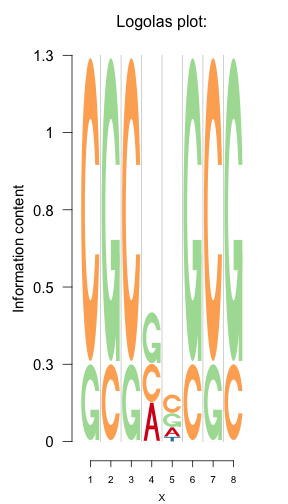
\includegraphics[width=6in,height=5in]{figure/standard_logo-1} 

\end{knitrout}
\end{center}
\end{figure}


\subsection{Different configurations of standard logo}

Logolas also allows the user to choose different colors, change the scale of the Y axis, normalize the height of the logos and also play around with the margins of the plot in the plotting region. We present a demonstration of these feature of \textbf{Logolas} in the example below. We also show in this example, how multi-panel Logolas plots can be created.

We first set up the multiple panels and then present the standard logo plots under different customizations.

\begin{knitrout}
\definecolor{shadecolor}{rgb}{0.969, 0.969, 0.969}\color{fgcolor}\begin{kframe}
\begin{alltt}
\hlcom{######################      Setting up multiple panels        ########################}

\hlkwd{library}\hlstd{(grid)}
\hlkwd{library}\hlstd{(gridBase)}
\hlkwd{library}\hlstd{(gridExtra)}

\hlkwd{grid.newpage}\hlstd{()}
\hlstd{layout.rows} \hlkwb{<-} \hlnum{2}
\hlstd{layout.cols} \hlkwb{<-} \hlnum{2}
\hlstd{top.vp} \hlkwb{<-} \hlkwd{viewport}\hlstd{(}\hlkwc{layout}\hlstd{=}\hlkwd{grid.layout}\hlstd{(layout.rows, layout.cols,}
                                      \hlkwc{widths}\hlstd{=}\hlkwd{unit}\hlstd{(}\hlkwd{rep}\hlstd{(}\hlnum{5}\hlstd{,layout.cols),} \hlkwd{rep}\hlstd{(}\hlstr{"null"}\hlstd{,} \hlnum{2}\hlstd{)),}
                                      \hlkwc{heights}\hlstd{=}\hlkwd{unit}\hlstd{(}\hlkwd{rep}\hlstd{(}\hlnum{5}\hlstd{,layout.rows),} \hlkwd{rep}\hlstd{(}\hlstr{"null"}\hlstd{,} \hlnum{1}\hlstd{))))}
\hlstd{plot_reg} \hlkwb{<-} \hlkwd{vpList}\hlstd{()}
\hlstd{l} \hlkwb{<-} \hlnum{1}
\hlkwa{for}\hlstd{(i} \hlkwa{in} \hlnum{1}\hlopt{:}\hlstd{layout.rows)\{}
  \hlkwa{for}\hlstd{(j} \hlkwa{in} \hlnum{1}\hlopt{:}\hlstd{layout.cols)\{}
    \hlstd{plot_reg[[l]]} \hlkwb{<-} \hlkwd{viewport}\hlstd{(}\hlkwc{layout.pos.col} \hlstd{= j,} \hlkwc{layout.pos.row} \hlstd{= i,} \hlkwc{name} \hlstd{=} \hlkwd{paste0}\hlstd{(}\hlstr{"plotlogo"}\hlstd{, l))}
    \hlstd{l} \hlkwb{<-} \hlstd{l}\hlopt{+}\hlnum{1}
  \hlstd{\}}
\hlstd{\}}


\hlstd{plot_tree} \hlkwb{<-} \hlkwd{vpTree}\hlstd{(top.vp, plot_reg)}

\hlkwd{pushViewport}\hlstd{(plot_tree)}


\hlcom{##########################   Creating the multi-panel logos   ##############################}


\hlcom{#change the color of letters}
\hlcom{#change the diverging palettes}
\hlstd{color_profile1}\hlkwb{=}\hlkwd{list}\hlstd{(}\hlstr{"type"} \hlstd{=} \hlstr{"per_row"}\hlstd{,}
\hlstr{"col"} \hlstd{= RColorBrewer}\hlopt{::}\hlkwd{brewer.pal}\hlstd{(}\hlkwd{dim}\hlstd{(}\hlkwd{attr}\hlstd{(p,} \hlstr{"pwm"}\hlstd{))[}\hlnum{1}\hlstd{],}\hlkwc{name} \hlstd{=}\hlstr{"PiYG"}\hlstd{))}
\hlkwd{seekViewport}\hlstd{(}\hlkwd{paste0}\hlstd{(}\hlstr{"plotlogo"}\hlstd{,} \hlnum{1}\hlstd{))}
\hlkwd{logomaker}\hlstd{(}\hlkwd{attr}\hlstd{(p,} \hlstr{"pwm"}\hlstd{),}\hlkwc{xlab} \hlstd{=} \hlstr{'position'}\hlstd{,}\hlkwc{color_profile} \hlstd{= color_profile1,}
          \hlkwc{frame_width} \hlstd{=} \hlnum{1}\hlstd{,}
          \hlkwc{newpage} \hlstd{=} \hlnum{FALSE}\hlstd{,}
          \hlkwc{pop_name} \hlstd{=} \hlstr{'Change color'}\hlstd{,}
          \hlkwc{control} \hlstd{=} \hlkwd{list}\hlstd{(}\hlkwc{viewport.margin.left} \hlstd{=} \hlnum{5}\hlstd{))}

\hlcom{#change the y scale:}
\hlcom{#if yscale_change = FALSE, then the height of y axis would be 2.}
\hlkwd{seekViewport}\hlstd{(}\hlkwd{paste0}\hlstd{(}\hlstr{"plotlogo"}\hlstd{,} \hlnum{2}\hlstd{))}
\hlkwd{logomaker}\hlstd{(}\hlkwd{attr}\hlstd{(p,} \hlstr{"pwm"}\hlstd{),}\hlkwc{xlab} \hlstd{=} \hlstr{'position'}\hlstd{,}\hlkwc{color_profile} \hlstd{= color_profile,}
          \hlkwc{frame_width} \hlstd{=} \hlnum{1}\hlstd{,}
          \hlkwc{newpage} \hlstd{=} \hlnum{FALSE}\hlstd{,}
          \hlkwc{pop_name} \hlstd{=} \hlstr{'Change y scale'}\hlstd{,}
          \hlkwc{yscale_change} \hlstd{=} \hlnum{FALSE}\hlstd{,}
          \hlkwc{control} \hlstd{=} \hlkwd{list}\hlstd{(}\hlkwc{viewport.margin.left} \hlstd{=} \hlnum{5}\hlstd{))}
\hlcom{#Normalize the height of bars to 1}
\hlkwd{seekViewport}\hlstd{(}\hlkwd{paste0}\hlstd{(}\hlstr{"plotlogo"}\hlstd{,} \hlnum{3}\hlstd{))}
\hlkwd{logomaker}\hlstd{(}\hlkwd{attr}\hlstd{(p,} \hlstr{"pwm"}\hlstd{),}\hlkwc{xlab} \hlstd{=} \hlstr{'position'}\hlstd{,}\hlkwc{color_profile} \hlstd{= color_profile,}
          \hlkwc{frame_width} \hlstd{=} \hlnum{1}\hlstd{,}
          \hlkwc{newpage} \hlstd{=} \hlnum{FALSE}\hlstd{,}
          \hlkwc{ic.scale} \hlstd{=} \hlnum{FALSE}\hlstd{,}
          \hlkwc{pop_name} \hlstd{=} \hlstr{'Normalize the height'}\hlstd{,}
          \hlkwc{control} \hlstd{=} \hlkwd{list}\hlstd{(}\hlkwc{viewport.margin.left} \hlstd{=} \hlnum{5}\hlstd{))}
\hlcom{#change the background probability}
\hlcom{#And modify the title and the axis label}
\hlkwd{seekViewport}\hlstd{(}\hlkwd{paste0}\hlstd{(}\hlstr{"plotlogo"}\hlstd{,} \hlnum{4}\hlstd{))}
\hlkwd{logomaker}\hlstd{(}\hlkwd{attr}\hlstd{(p,} \hlstr{"pwm"}\hlstd{),}\hlkwc{xlab} \hlstd{=} \hlstr{'position'}\hlstd{,}\hlkwc{color_profile} \hlstd{= color_profile,}
          \hlkwc{frame_width} \hlstd{=} \hlnum{1}\hlstd{,}
          \hlkwc{bg}\hlstd{=}\hlkwd{c}\hlstd{(}\hlnum{0.32}\hlstd{,} \hlnum{0.18}\hlstd{,} \hlnum{0.2}\hlstd{,} \hlnum{0.3}\hlstd{),}
          \hlkwc{newpage} \hlstd{=} \hlnum{FALSE}\hlstd{,}
          \hlkwc{pop_name} \hlstd{=} \hlstr{'Change background prob'}\hlstd{,}
          \hlkwc{control} \hlstd{=} \hlkwd{list}\hlstd{(}\hlkwc{viewport.margin.left} \hlstd{=} \hlnum{5}\hlstd{))}
\end{alltt}
\end{kframe}
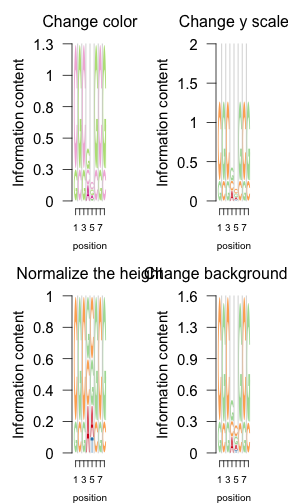
\includegraphics[width=6in,height=5in]{figure/diff_features-1} 

\end{knitrout}

% \begin{figure}[h]
% \begin{center}
% 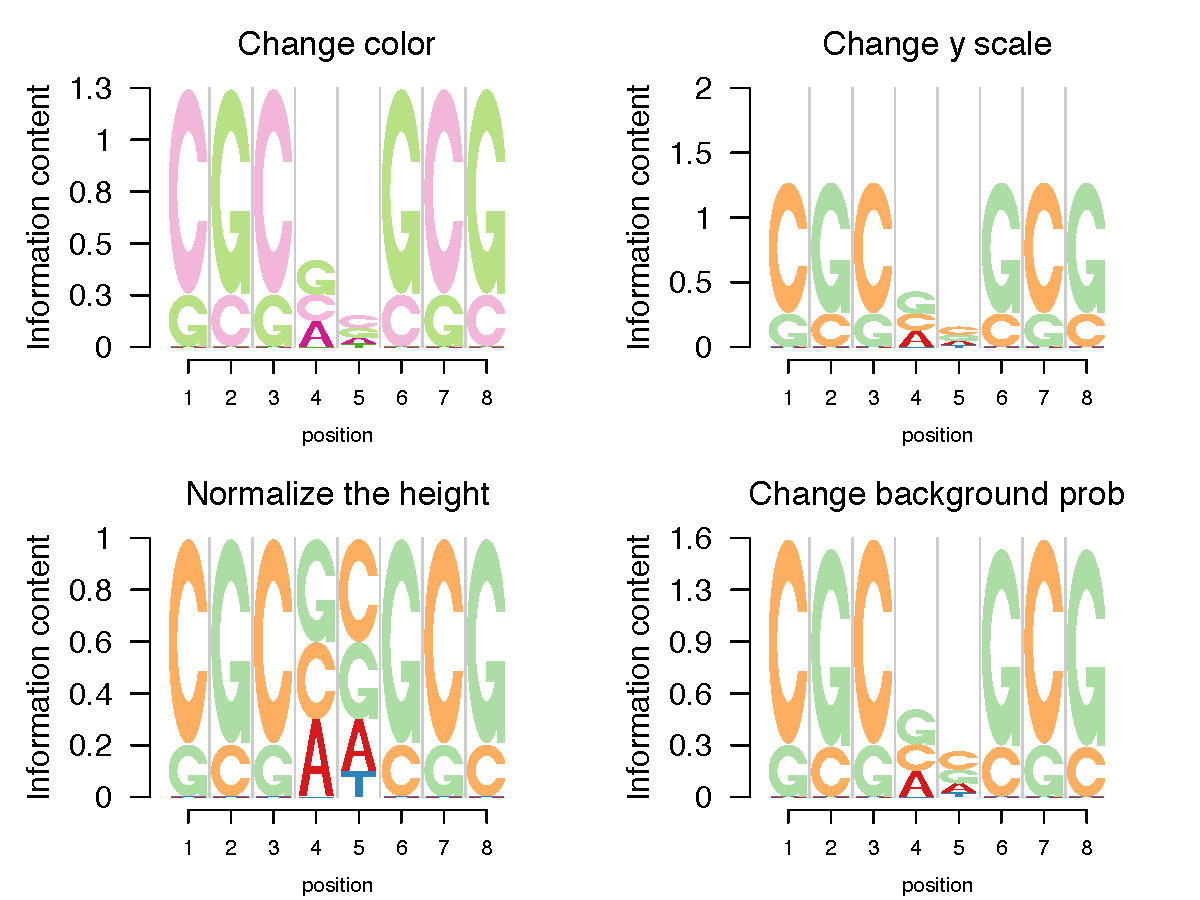
\includegraphics[height=6in, width=8in]{figure/panel1.pdf}
% \end{center}
% \end{figure}

\subsection{Other entropy measures}

Besides the default Shannon entropy, \textit{logomaker} function in
textbf{Logolas} can also determine the Information Criterion using Renyi entrop. For this entropy measure, the Information content at position $i$ is $IC_{i,\alpha}=\frac{1}{1-\alpha}\Sigma_b\log_2(q_{b,i}^\alpha-0.25^{1-\alpha})$. When $\alpha\rightarrow1$, the limiting value of Renyi entropy is the Shannon entropy. In `logomaker`, `alpha` is a control parameter that can be tuned to get plots for different entropy measures. The figure below shows the logo plots with different values of $\alpha$.

\begin{knitrout}
\definecolor{shadecolor}{rgb}{0.969, 0.969, 0.969}\color{fgcolor}\begin{kframe}
\begin{alltt}
\hlkwd{grid.newpage}\hlstd{()}
\hlstd{layout.rows} \hlkwb{<-} \hlnum{1}
\hlstd{layout.cols} \hlkwb{<-} \hlnum{2}
\hlstd{top.vp} \hlkwb{<-} \hlkwd{viewport}\hlstd{(}\hlkwc{layout}\hlstd{=}\hlkwd{grid.layout}\hlstd{(layout.rows, layout.cols,}
                                      \hlkwc{widths}\hlstd{=}\hlkwd{unit}\hlstd{(}\hlkwd{rep}\hlstd{(}\hlnum{6}\hlstd{,layout.cols),} \hlkwd{rep}\hlstd{(}\hlstr{"null"}\hlstd{,} \hlnum{2}\hlstd{)),}
                                      \hlkwc{heights}\hlstd{=}\hlkwd{unit}\hlstd{(}\hlkwd{c}\hlstd{(}\hlnum{20}\hlstd{,}\hlnum{20}\hlstd{),} \hlkwd{rep}\hlstd{(}\hlstr{"lines"}\hlstd{,} \hlnum{2}\hlstd{))))}

\hlstd{plot_reg} \hlkwb{<-} \hlkwd{vpList}\hlstd{()}
\hlstd{l} \hlkwb{<-} \hlnum{1}
\hlkwa{for}\hlstd{(i} \hlkwa{in} \hlnum{1}\hlopt{:}\hlstd{layout.rows)\{}
  \hlkwa{for}\hlstd{(j} \hlkwa{in} \hlnum{1}\hlopt{:}\hlstd{layout.cols)\{}
    \hlstd{plot_reg[[l]]} \hlkwb{<-} \hlkwd{viewport}\hlstd{(}\hlkwc{layout.pos.col} \hlstd{= j,} \hlkwc{layout.pos.row} \hlstd{= i,} \hlkwc{name} \hlstd{=} \hlkwd{paste0}\hlstd{(}\hlstr{"plotlogo"}\hlstd{, l))}
    \hlstd{l} \hlkwb{<-} \hlstd{l}\hlopt{+}\hlnum{1}
  \hlstd{\}}
\hlstd{\}}


\hlstd{plot_tree} \hlkwb{<-} \hlkwd{vpTree}\hlstd{(top.vp, plot_reg)}

\hlkwd{pushViewport}\hlstd{(plot_tree)}
\hlkwd{seekViewport}\hlstd{(}\hlkwd{paste0}\hlstd{(}\hlstr{"plotlogo"}\hlstd{,} \hlnum{1}\hlstd{))}
\hlkwd{logomaker}\hlstd{(}\hlkwd{attr}\hlstd{(p,} \hlstr{"pwm"}\hlstd{),}\hlkwc{xlab} \hlstd{=} \hlstr{'position'}\hlstd{,}\hlkwc{color_profile} \hlstd{= color_profile,}
          \hlkwc{frame_width} \hlstd{=} \hlnum{1}\hlstd{,}
          \hlkwc{newpage} \hlstd{=} \hlnum{FALSE}\hlstd{,}
          \hlkwc{pop_name} \hlstd{=} \hlstr{'Logo plot, Alpha=2'}\hlstd{,}
          \hlkwc{control} \hlstd{=} \hlkwd{list}\hlstd{(}\hlkwc{viewport.margin.left} \hlstd{=} \hlnum{5}\hlstd{,}\hlkwc{alpha}\hlstd{=}\hlnum{2}\hlstd{))}


\hlkwd{seekViewport}\hlstd{(}\hlkwd{paste0}\hlstd{(}\hlstr{"plotlogo"}\hlstd{,} \hlnum{2}\hlstd{))}
\hlkwd{logomaker}\hlstd{(}\hlkwd{attr}\hlstd{(p,} \hlstr{"pwm"}\hlstd{),}\hlkwc{xlab} \hlstd{=} \hlstr{'position'}\hlstd{,}\hlkwc{color_profile} \hlstd{= color_profile,}
          \hlkwc{frame_width} \hlstd{=} \hlnum{1}\hlstd{,}
          \hlkwc{newpage} \hlstd{=} \hlnum{FALSE}\hlstd{,}
          \hlkwc{pop_name} \hlstd{=} \hlstr{'Logo plot, Alpha=0.2'}\hlstd{,}
          \hlkwc{control} \hlstd{=} \hlkwd{list}\hlstd{(}\hlkwc{viewport.margin.left} \hlstd{=} \hlnum{5}\hlstd{,}\hlkwc{alpha}\hlstd{=}\hlnum{0.2}\hlstd{))}
\end{alltt}
\end{kframe}
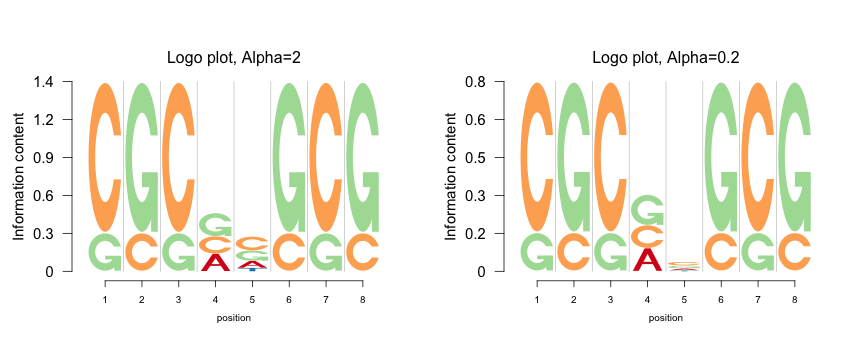
\includegraphics[width=6in,height=5in]{figure/entropy-1} 

\end{knitrout}


\subsection{Combine Logolas with ggplot2}

The user can also embed the Logolas plots with ggplot2 graphics. We present a simple illustration below.

\begin{knitrout}
\definecolor{shadecolor}{rgb}{0.969, 0.969, 0.969}\color{fgcolor}\begin{kframe}
\begin{alltt}
\hlkwd{library}\hlstd{(ggplot2)}
\hlkwd{library}\hlstd{(grid)}
\hlkwd{library}\hlstd{(gridBase)}


\hlkwd{grid.newpage}\hlstd{()}
\hlstd{layout.rows} \hlkwb{<-} \hlnum{1}
\hlstd{layout.cols} \hlkwb{<-} \hlnum{2}
\hlstd{top.vp} \hlkwb{<-} \hlkwd{viewport}\hlstd{(}\hlkwc{layout}\hlstd{=}\hlkwd{grid.layout}\hlstd{(layout.rows, layout.cols,}
                                      \hlkwc{widths}\hlstd{=}\hlkwd{unit}\hlstd{(}\hlkwd{rep}\hlstd{(}\hlnum{6}\hlstd{,layout.cols),} \hlkwd{rep}\hlstd{(}\hlstr{"null"}\hlstd{, layout.cols)),}
                                      \hlkwc{heights}\hlstd{=}\hlkwd{unit}\hlstd{(}\hlkwd{rep}\hlstd{(}\hlnum{20}\hlstd{,}\hlnum{20}\hlstd{),} \hlkwd{rep}\hlstd{(}\hlstr{"null"}\hlstd{,}\hlnum{1}\hlstd{))))}

\hlstd{plot_reg} \hlkwb{<-} \hlkwd{vpList}\hlstd{()}
\hlstd{l} \hlkwb{<-} \hlnum{1}
\hlkwa{for}\hlstd{(i} \hlkwa{in} \hlnum{1}\hlopt{:}\hlstd{layout.rows)\{}
  \hlkwa{for}\hlstd{(j} \hlkwa{in} \hlnum{1}\hlopt{:}\hlstd{layout.cols)\{}
    \hlstd{plot_reg[[l]]} \hlkwb{<-} \hlkwd{viewport}\hlstd{(}\hlkwc{layout.pos.col} \hlstd{= j,} \hlkwc{layout.pos.row} \hlstd{= i,} \hlkwc{name} \hlstd{=} \hlkwd{paste0}\hlstd{(}\hlstr{"plotlogo"}\hlstd{, l))}
    \hlstd{l} \hlkwb{<-} \hlstd{l}\hlopt{+}\hlnum{1}
  \hlstd{\}}
\hlstd{\}}


\hlstd{plot_tree} \hlkwb{<-} \hlkwd{vpTree}\hlstd{(top.vp, plot_reg)}

\hlkwd{pushViewport}\hlstd{(plot_tree)}
\hlkwd{seekViewport}\hlstd{(}\hlkwd{paste0}\hlstd{(}\hlstr{"plotlogo"}\hlstd{,} \hlnum{1}\hlstd{))}
\hlkwd{logomaker}\hlstd{(}\hlkwd{attr}\hlstd{(p,} \hlstr{"pwm"}\hlstd{),}\hlkwc{xlab} \hlstd{=} \hlstr{'position'}\hlstd{,}\hlkwc{color_profile} \hlstd{= color_profile,}
          \hlkwc{bg} \hlstd{=} \hlkwd{c}\hlstd{(}\hlnum{0.28}\hlstd{,} \hlnum{0.22}\hlstd{,} \hlnum{0.24}\hlstd{,} \hlnum{0.26}\hlstd{),}
          \hlkwc{frame_width} \hlstd{=} \hlnum{1}\hlstd{,}
          \hlkwc{newpage} \hlstd{=} \hlnum{FALSE}\hlstd{,}
          \hlkwc{control} \hlstd{=} \hlkwd{list}\hlstd{(}\hlkwc{viewport.margin.left} \hlstd{=} \hlnum{5}\hlstd{))}


\hlkwd{seekViewport}\hlstd{(}\hlkwd{paste0}\hlstd{(}\hlstr{"plotlogo"}\hlstd{,} \hlnum{2}\hlstd{))}
\hlstd{vp3} \hlkwb{=} \hlkwd{viewport}\hlstd{(}\hlkwc{width}\hlstd{=}\hlnum{0.8}\hlstd{,} \hlkwc{height}\hlstd{=}\hlnum{0.8}\hlstd{,} \hlkwc{x} \hlstd{=} \hlnum{0.5}\hlstd{,} \hlkwc{y} \hlstd{=} \hlnum{0.5}\hlstd{)}
\hlstd{p} \hlkwb{<-} \hlkwd{qplot}\hlstd{(mpg,} \hlkwc{data}\hlstd{=mtcars,} \hlkwc{geom}\hlstd{=}\hlstr{"density"}\hlstd{)}
\hlkwd{print}\hlstd{(p,} \hlkwc{vp} \hlstd{= vp3)}
\end{alltt}
\end{kframe}
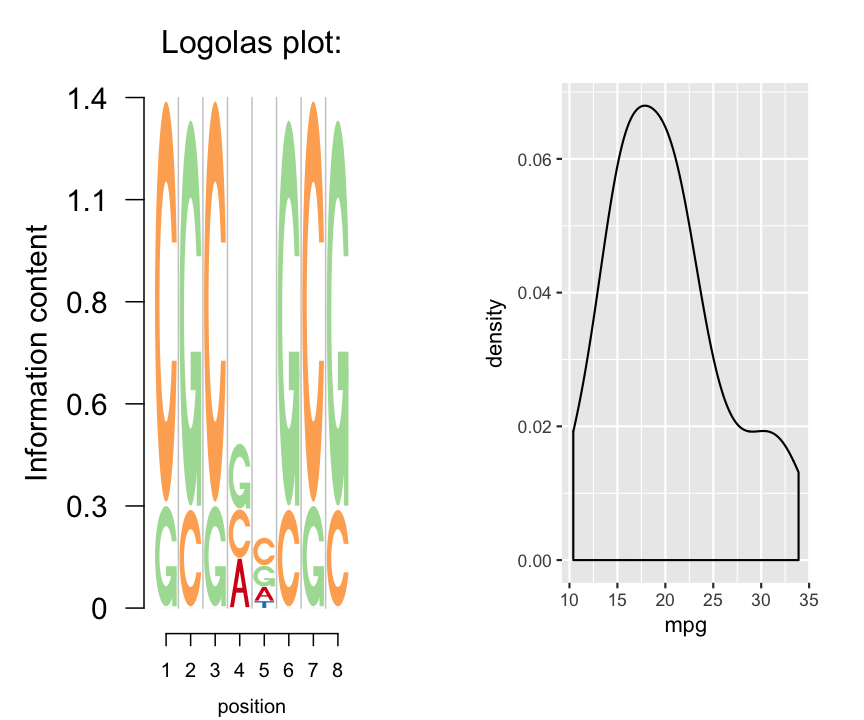
\includegraphics[width=6in,height=5in]{figure/ggplot2-1} 

\end{knitrout}

\section{EDLogo Representation}

Standard sequence logos tend to highlight the enrichment of symbols. In this esection, we introduce \textit{EDLogo}, an alternative visualization to the standard sequence logos that highlights both enrichment and depletion.

For example, suppose for a particular position, the base composition of $ \left (A, C, G, T \right)$ is as follows

$$ \left (A, C, G, T \right ) : = \left ( 0.33, 0.33, 0.01, 0.33 \right )  $$

Sequence logos will show a mild enrichment of A, C, G in this position and the stack height for this position will be relativelys small compared to the ones with enrichment. This generally makes it hard to see the depletion. \textit{EDLogo} is a solution to this problem. We illustrate that with an example compariosn of \textit{EDLogo} and standard sequence logo below.

\subsection{EDLogo - First example}


\begin{knitrout}
\definecolor{shadecolor}{rgb}{0.969, 0.969, 0.969}\color{fgcolor}\begin{kframe}
\begin{alltt}
\hlkwd{library}\hlstd{(ggplot2)}
\hlkwd{library}\hlstd{(grid)}
\hlkwd{library}\hlstd{(gridBase)}


\hlkwd{grid.newpage}\hlstd{()}
\hlstd{layout.rows} \hlkwb{<-} \hlnum{1}
\hlstd{layout.cols} \hlkwb{<-} \hlnum{2}
\hlstd{top.vp} \hlkwb{<-} \hlkwd{viewport}\hlstd{(}\hlkwc{layout}\hlstd{=}\hlkwd{grid.layout}\hlstd{(layout.rows, layout.cols,}
                                      \hlkwc{widths}\hlstd{=}\hlkwd{unit}\hlstd{(}\hlkwd{rep}\hlstd{(}\hlnum{6}\hlstd{,layout.cols),} \hlkwd{rep}\hlstd{(}\hlstr{"null"}\hlstd{, layout.cols)),}
                                      \hlkwc{heights}\hlstd{=}\hlkwd{unit}\hlstd{(}\hlkwd{rep}\hlstd{(}\hlnum{20}\hlstd{,}\hlnum{20}\hlstd{),} \hlkwd{rep}\hlstd{(}\hlstr{"null"}\hlstd{,}\hlnum{1}\hlstd{))))}

\hlstd{plot_reg} \hlkwb{<-} \hlkwd{vpList}\hlstd{()}
\hlstd{l} \hlkwb{<-} \hlnum{1}
\hlkwa{for}\hlstd{(i} \hlkwa{in} \hlnum{1}\hlopt{:}\hlstd{layout.rows)\{}
  \hlkwa{for}\hlstd{(j} \hlkwa{in} \hlnum{1}\hlopt{:}\hlstd{layout.cols)\{}
    \hlstd{plot_reg[[l]]} \hlkwb{<-} \hlkwd{viewport}\hlstd{(}\hlkwc{layout.pos.col} \hlstd{= j,} \hlkwc{layout.pos.row} \hlstd{= i,} \hlkwc{name} \hlstd{=} \hlkwd{paste0}\hlstd{(}\hlstr{"plotlogo"}\hlstd{, l))}
    \hlstd{l} \hlkwb{<-} \hlstd{l}\hlopt{+}\hlnum{1}
  \hlstd{\}}
\hlstd{\}}

\hlstd{plot_tree} \hlkwb{<-} \hlkwd{vpTree}\hlstd{(top.vp, plot_reg)}

\hlkwd{pushViewport}\hlstd{(plot_tree)}

\hlstd{pwm}\hlkwb{=}\hlkwd{cbind}\hlstd{(}\hlkwd{c}\hlstd{(}\hlnum{1}\hlstd{,}\hlnum{0}\hlstd{,}\hlnum{0}\hlstd{,}\hlnum{0}\hlstd{),}\hlkwd{c}\hlstd{(}\hlnum{0.328}\hlstd{,}\hlnum{0.332}\hlstd{,}\hlnum{0.33}\hlstd{,}\hlnum{0.01}\hlstd{),}
          \hlkwd{c}\hlstd{(}\hlnum{0.1}\hlstd{,}\hlnum{0.8}\hlstd{,}\hlnum{0.05}\hlstd{,}\hlnum{0.05}\hlstd{),}\hlkwd{c}\hlstd{(}\hlnum{0}\hlstd{,}\hlnum{0.05}\hlstd{,}\hlnum{0.95}\hlstd{,}\hlnum{0}\hlstd{))}
\hlkwd{rownames}\hlstd{(pwm)}\hlkwb{=}\hlkwd{c}\hlstd{(}\hlstr{'A'}\hlstd{,}\hlstr{'C'}\hlstd{,}\hlstr{'G'}\hlstd{,}\hlstr{'T'}\hlstd{)}
\hlkwd{colnames}\hlstd{(pwm)}\hlkwb{=}\hlnum{1}\hlopt{:}\hlkwd{ncol}\hlstd{(pwm)}

\hlkwd{seekViewport}\hlstd{(}\hlkwd{paste0}\hlstd{(}\hlstr{"plotlogo"}\hlstd{,} \hlnum{1}\hlstd{))}
\hlkwd{logomaker}\hlstd{(pwm,}\hlkwc{color_profile}\hlstd{=color_profile,}\hlkwc{frame_width} \hlstd{=} \hlnum{1}\hlstd{,}\hlkwc{pop_name} \hlstd{=} \hlstr{'Logo'}\hlstd{,}\hlkwc{control} \hlstd{=} \hlkwd{list}\hlstd{(}\hlkwc{gap_ylab}\hlstd{=}\hlnum{3.5}\hlstd{),} \hlkwc{newpage} \hlstd{=} \hlnum{FALSE}\hlstd{)}

\hlkwd{seekViewport}\hlstd{(}\hlkwd{paste0}\hlstd{(}\hlstr{"plotlogo"}\hlstd{,} \hlnum{2}\hlstd{))}
\hlkwd{nlogomaker}\hlstd{(pwm,}\hlkwc{logoheight} \hlstd{=} \hlstr{'log'}\hlstd{,}\hlkwc{color_profile} \hlstd{= color_profile,}\hlkwc{pop_name} \hlstd{=} \hlstr{'EDLogo'}\hlstd{,}\hlkwc{control} \hlstd{=} \hlkwd{list}\hlstd{(}\hlkwc{gap_ylab}\hlstd{=}\hlnum{3.5}\hlstd{),} \hlkwc{newpage} \hlstd{=} \hlnum{FALSE}\hlstd{)}
\end{alltt}
\end{kframe}
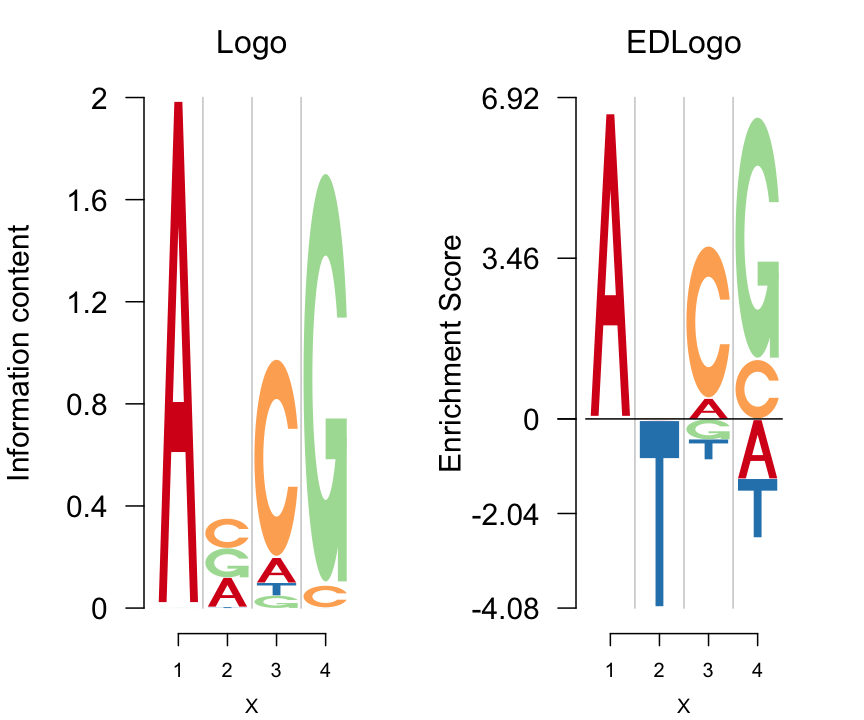
\includegraphics[width=6in,height=5in]{figure/edlogo-1} 

\end{knitrout}


\subsection{Different options of EDLogo}

The \textit{EDLogo} plot is created using the \textit{nlogomaker} function. Note that there is a \textit{logoheight} option in this plot which was set to \textit{log} for the above example. Actually there are total $8$ options for \textit{logoheight} - the details can be found in Documentation. A comparative analysis of some of these options on the seqLogo example is provided below.


\begin{knitrout}
\definecolor{shadecolor}{rgb}{0.969, 0.969, 0.969}\color{fgcolor}\begin{kframe}
\begin{alltt}
\hlstd{mFile} \hlkwb{<-} \hlkwd{system.file}\hlstd{(}\hlstr{"Exfiles/pwm1"}\hlstd{,} \hlkwc{package}\hlstd{=}\hlstr{"seqLogo"}\hlstd{)}
\hlstd{m} \hlkwb{<-} \hlkwd{read.table}\hlstd{(mFile)}
\hlstd{p} \hlkwb{<-} \hlstd{seqLogo}\hlopt{::}\hlkwd{makePWM}\hlstd{(m)}

\hlkwd{grid.newpage}\hlstd{()}
\hlstd{layout.rows} \hlkwb{<-} \hlnum{2}
\hlstd{layout.cols} \hlkwb{<-} \hlnum{2}
\hlstd{top.vp} \hlkwb{<-} \hlkwd{viewport}\hlstd{(}\hlkwc{layout}\hlstd{=}\hlkwd{grid.layout}\hlstd{(layout.rows, layout.cols,}
                                      \hlkwc{widths}\hlstd{=}\hlkwd{unit}\hlstd{(}\hlkwd{rep}\hlstd{(}\hlnum{5}\hlstd{,layout.cols),} \hlkwd{rep}\hlstd{(}\hlstr{"null"}\hlstd{,} \hlnum{2}\hlstd{)),}
                                      \hlkwc{heights}\hlstd{=}\hlkwd{unit}\hlstd{(}\hlkwd{rep}\hlstd{(}\hlnum{5}\hlstd{,layout.rows),} \hlkwd{rep}\hlstd{(}\hlstr{"null"}\hlstd{,} \hlnum{1}\hlstd{))))}
\hlstd{plot_reg} \hlkwb{<-} \hlkwd{vpList}\hlstd{()}
\hlstd{l} \hlkwb{<-} \hlnum{1}
\hlkwa{for}\hlstd{(i} \hlkwa{in} \hlnum{1}\hlopt{:}\hlstd{layout.rows)\{}
  \hlkwa{for}\hlstd{(j} \hlkwa{in} \hlnum{1}\hlopt{:}\hlstd{layout.cols)\{}
    \hlstd{plot_reg[[l]]} \hlkwb{<-} \hlkwd{viewport}\hlstd{(}\hlkwc{layout.pos.col} \hlstd{= j,} \hlkwc{layout.pos.row} \hlstd{= i,} \hlkwc{name} \hlstd{=} \hlkwd{paste0}\hlstd{(}\hlstr{"plotlogo"}\hlstd{, l))}
    \hlstd{l} \hlkwb{<-} \hlstd{l}\hlopt{+}\hlnum{1}
  \hlstd{\}}
\hlstd{\}}


\hlstd{plot_tree} \hlkwb{<-} \hlkwd{vpTree}\hlstd{(top.vp, plot_reg)}

\hlkwd{pushViewport}\hlstd{(plot_tree)}
\hlkwd{seekViewport}\hlstd{(}\hlkwd{paste0}\hlstd{(}\hlstr{"plotlogo"}\hlstd{,} \hlnum{1}\hlstd{))}
\hlkwd{nlogomaker}\hlstd{(}\hlkwd{attr}\hlstd{(p,} \hlstr{"pwm"}\hlstd{),}\hlkwc{logoheight} \hlstd{=} \hlstr{'log'}\hlstd{,}\hlkwc{color_profile} \hlstd{= color_profile,}\hlkwc{frame_width} \hlstd{=} \hlnum{1}\hlstd{,} \hlkwc{pop_name} \hlstd{=} \hlstr{"log"}\hlstd{,} \hlkwc{newpage} \hlstd{=} \hlnum{FALSE}\hlstd{)}


\hlkwd{seekViewport}\hlstd{(}\hlkwd{paste0}\hlstd{(}\hlstr{"plotlogo"}\hlstd{,} \hlnum{2}\hlstd{))}
\hlkwd{nlogomaker}\hlstd{(}\hlkwd{attr}\hlstd{(p,} \hlstr{"pwm"}\hlstd{),}\hlkwc{logoheight} \hlstd{=} \hlstr{'log_odds'}\hlstd{,}\hlkwc{color_profile} \hlstd{= color_profile,}\hlkwc{frame_width} \hlstd{=} \hlnum{1}\hlstd{,} \hlkwc{pop_name} \hlstd{=} \hlstr{"log_odds"}\hlstd{,} \hlkwc{newpage} \hlstd{=} \hlnum{FALSE}\hlstd{)}

\hlkwd{seekViewport}\hlstd{(}\hlkwd{paste0}\hlstd{(}\hlstr{"plotlogo"}\hlstd{,} \hlnum{3}\hlstd{))}
\hlkwd{nlogomaker}\hlstd{(}\hlkwd{attr}\hlstd{(p,} \hlstr{"pwm"}\hlstd{),}\hlkwc{logoheight} \hlstd{=} \hlstr{'ratio'}\hlstd{,}\hlkwc{color_profile} \hlstd{= color_profile,}\hlkwc{frame_width} \hlstd{=} \hlnum{1}\hlstd{,} \hlkwc{pop_name} \hlstd{=} \hlstr{"ratio"}\hlstd{,} \hlkwc{newpage} \hlstd{=} \hlnum{FALSE}\hlstd{)}
\end{alltt}
\end{kframe}
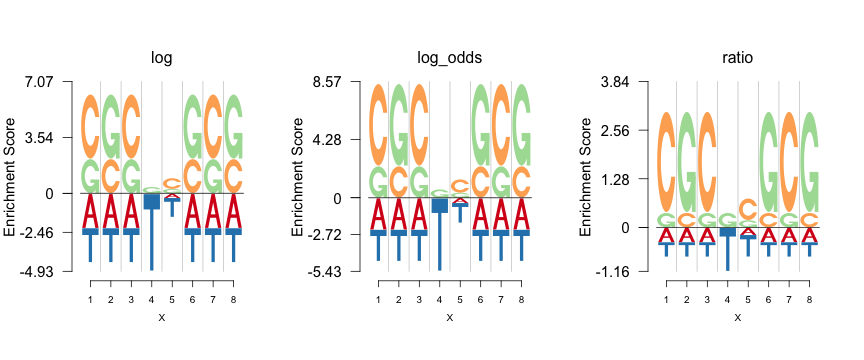
\includegraphics[width=6in,height=5in]{figure/edlogo_opts-1} 

\end{knitrout}



\section{Applications}

We present some examples beyond the DNA, RNA sequence motif examples that we dealt with thus far.

\subsection{Amino acid sequence motif}

One can use \Logolas{} for amino acid sequence motif detection as well, as the logo library of the software includes all the English alphabets and the 20 amino acids have a 1-letter representation using English alphabets.


\begin{knitrout}
\definecolor{shadecolor}{rgb}{0.969, 0.969, 0.969}\color{fgcolor}\begin{kframe}
\begin{alltt}
\hlstd{counts_mat} \hlkwb{<-} \hlkwd{rbind}\hlstd{(}\hlkwd{c}\hlstd{(}\hlnum{0}\hlstd{,} \hlnum{0}\hlstd{,} \hlnum{100}\hlstd{,} \hlnum{1}\hlstd{,} \hlnum{2}\hlstd{),} \hlkwd{c}\hlstd{(}\hlnum{4}\hlstd{,} \hlnum{3}\hlstd{,} \hlnum{30}\hlstd{,} \hlnum{35}\hlstd{,} \hlnum{2}\hlstd{),}
                    \hlkwd{c}\hlstd{(}\hlnum{100}\hlstd{,} \hlnum{0}\hlstd{,} \hlnum{10}\hlstd{,} \hlnum{2}\hlstd{,} \hlnum{7}\hlstd{),}\hlkwd{rep}\hlstd{(}\hlnum{0}\hlstd{,}\hlnum{5}\hlstd{),}
                    \hlkwd{c}\hlstd{(}\hlnum{4}\hlstd{,} \hlnum{2}\hlstd{,} \hlnum{3}\hlstd{,} \hlnum{7}\hlstd{,} \hlnum{70}\hlstd{),} \hlkwd{c}\hlstd{(}\hlnum{1}\hlstd{,} \hlnum{8}\hlstd{,} \hlnum{0}\hlstd{,} \hlnum{60}\hlstd{,} \hlnum{3}\hlstd{),}
                    \hlkwd{rep}\hlstd{(}\hlnum{0}\hlstd{,} \hlnum{5}\hlstd{),} \hlkwd{c}\hlstd{(}\hlnum{4}\hlstd{,} \hlnum{2}\hlstd{,} \hlnum{100}\hlstd{,} \hlnum{1}\hlstd{,} \hlnum{1}\hlstd{),}
                    \hlkwd{c}\hlstd{(}\hlnum{12}\hlstd{,} \hlnum{8}\hlstd{,} \hlnum{16}\hlstd{,} \hlnum{7}\hlstd{,} \hlnum{20}\hlstd{),} \hlkwd{c}\hlstd{(}\hlnum{55}\hlstd{,} \hlnum{0}\hlstd{,} \hlnum{1}\hlstd{,} \hlnum{0}\hlstd{,} \hlnum{12}\hlstd{),}
                    \hlkwd{rep}\hlstd{(}\hlnum{0}\hlstd{,}\hlnum{5}\hlstd{),} \hlkwd{c}\hlstd{(}\hlkwd{rep}\hlstd{(}\hlnum{0}\hlstd{,}\hlnum{3}\hlstd{),} \hlnum{20}\hlstd{,} \hlnum{0}\hlstd{),}
                    \hlkwd{rep}\hlstd{(}\hlnum{0}\hlstd{,}\hlnum{5}\hlstd{),} \hlkwd{c}\hlstd{(}\hlnum{0}\hlstd{,} \hlnum{0}\hlstd{,} \hlnum{30}\hlstd{,} \hlnum{0}\hlstd{,} \hlnum{22}\hlstd{),}
                    \hlkwd{c}\hlstd{(}\hlnum{1}\hlstd{,} \hlnum{0}\hlstd{,} \hlnum{12}\hlstd{,} \hlnum{3}\hlstd{,} \hlnum{10}\hlstd{),} \hlkwd{rep}\hlstd{(}\hlnum{0}\hlstd{,}\hlnum{5}\hlstd{),}
                    \hlkwd{c}\hlstd{(}\hlnum{0}\hlstd{,} \hlnum{1}\hlstd{,} \hlnum{0}\hlstd{,} \hlnum{34}\hlstd{,} \hlnum{1}\hlstd{),} \hlkwd{c}\hlstd{(}\hlnum{0}\hlstd{,} \hlnum{1}\hlstd{,} \hlnum{12}\hlstd{,} \hlnum{35}\hlstd{,} \hlnum{1}\hlstd{),}
                    \hlkwd{c}\hlstd{(}\hlnum{0}\hlstd{,} \hlnum{30}\hlstd{,} \hlnum{1}\hlstd{,} \hlnum{10}\hlstd{,} \hlnum{2}\hlstd{),} \hlkwd{c}\hlstd{(}\hlnum{0}\hlstd{,} \hlnum{1}\hlstd{,} \hlnum{4}\hlstd{,} \hlnum{100}\hlstd{,} \hlnum{2}\hlstd{))}
\end{alltt}
\end{kframe}
\end{knitrout}


\begin{figure}[htp]
\begin{center}
\begin{knitrout}
\definecolor{shadecolor}{rgb}{0.969, 0.969, 0.969}\color{fgcolor}\begin{kframe}
\begin{alltt}
\hlkwd{rownames}\hlstd{(counts_mat)} \hlkwb{<-} \hlkwd{c}\hlstd{(}\hlstr{"A"}\hlstd{,} \hlstr{"R"}\hlstd{,} \hlstr{"N"}\hlstd{,} \hlstr{"D"}\hlstd{,}\hlstr{"C"}\hlstd{,} \hlstr{"E"}\hlstd{,} \hlstr{"Q"}\hlstd{,} \hlstr{"G"}\hlstd{,}
                          \hlstr{"H"}\hlstd{,} \hlstr{"I"}\hlstd{,} \hlstr{"L"}\hlstd{,} \hlstr{"K"}\hlstd{,} \hlstr{"M"}\hlstd{,} \hlstr{"F"}\hlstd{,} \hlstr{"P"}\hlstd{,} \hlstr{"S"}\hlstd{,}
                          \hlstr{"T"}\hlstd{,} \hlstr{"W"}\hlstd{,} \hlstr{"Y"}\hlstd{,} \hlstr{"V"}\hlstd{)}

\hlkwd{colnames}\hlstd{(counts_mat)} \hlkwb{<-} \hlkwd{c}\hlstd{(}\hlstr{"Pos 1"}\hlstd{,} \hlstr{"Pos 2"}\hlstd{,} \hlstr{"Pos 3"}\hlstd{,} \hlstr{"Pos 4"}\hlstd{,} \hlstr{"Pos 5"}\hlstd{)}

\hlstd{cols1} \hlkwb{<-} \hlkwd{c}\hlstd{(}\hlkwd{rev}\hlstd{(RColorBrewer}\hlopt{::}\hlkwd{brewer.pal}\hlstd{(}\hlnum{12}\hlstd{,} \hlstr{"Paired"}\hlstd{))[}\hlkwd{c}\hlstd{(}\hlnum{3}\hlstd{,}\hlnum{4}\hlstd{,}\hlnum{7}\hlstd{,}\hlnum{8}\hlstd{,}\hlnum{11}\hlstd{,}\hlnum{12}\hlstd{,}\hlnum{5}\hlstd{,}\hlnum{6}\hlstd{,}\hlnum{9}\hlstd{,}\hlnum{10}\hlstd{)],}
           \hlstd{RColorBrewer}\hlopt{::}\hlkwd{brewer.pal}\hlstd{(}\hlnum{12}\hlstd{,} \hlstr{"Set3"}\hlstd{)[}\hlkwd{c}\hlstd{(}\hlnum{1}\hlstd{,}\hlnum{2}\hlstd{,}\hlnum{5}\hlstd{,}\hlnum{8}\hlstd{,}\hlnum{9}\hlstd{)],}
           \hlstd{RColorBrewer}\hlopt{::}\hlkwd{brewer.pal}\hlstd{(}\hlnum{9}\hlstd{,} \hlstr{"Set1"}\hlstd{)[}\hlkwd{c}\hlstd{(}\hlnum{9}\hlstd{,}\hlnum{7}\hlstd{)],}
           \hlstd{RColorBrewer}\hlopt{::}\hlkwd{brewer.pal}\hlstd{(}\hlnum{8}\hlstd{,} \hlstr{"Dark2"}\hlstd{)[}\hlkwd{c}\hlstd{(}\hlnum{3}\hlstd{,}\hlnum{4}\hlstd{,}\hlnum{8}\hlstd{)])}

\hlstd{color_profile} \hlkwb{<-} \hlkwd{list}\hlstd{(}\hlstr{"type"} \hlstd{=} \hlstr{"per_row"}\hlstd{,}
                      \hlstr{"col"} \hlstd{= cols1)}

\hlkwd{logomaker}\hlstd{(counts_mat,}
          \hlkwc{color_profile} \hlstd{= color_profile,}
          \hlkwc{frame_width} \hlstd{=} \hlnum{1}\hlstd{,}
          \hlkwc{ic.scale}  \hlstd{=} \hlnum{FALSE}\hlstd{,}
          \hlkwc{yscale_change} \hlstd{=} \hlnum{FALSE}\hlstd{)}
\end{alltt}
\end{kframe}
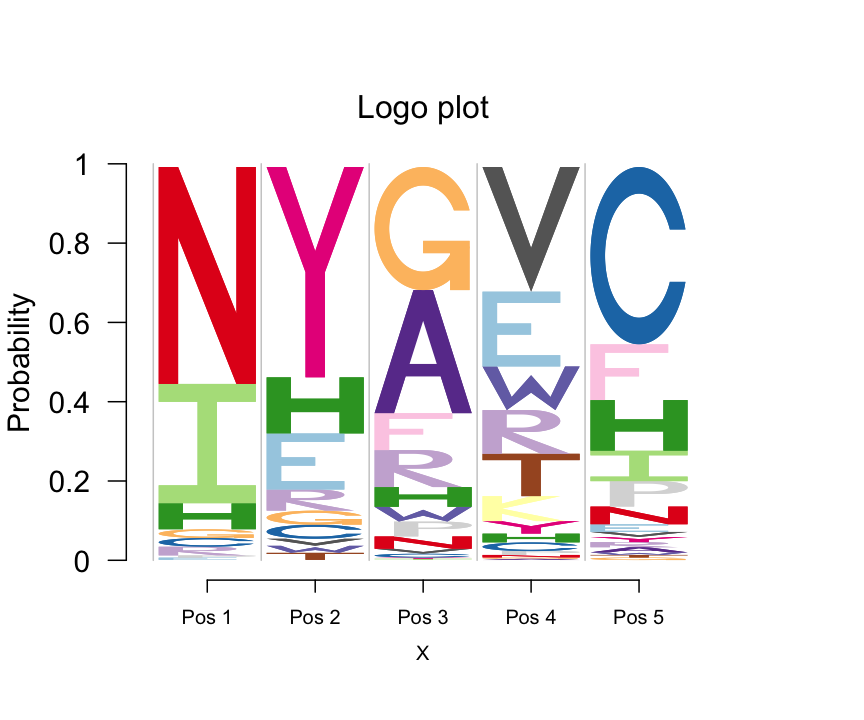
\includegraphics[width=6in,height=5in]{figure/logolas_use_5-1} 

\end{knitrout}
\end{center}
\end{figure}

Note that all one needs to do to build the logo plots is to specify the row names and column names as per the the logos and the stack labels and then fix the colors for the logos.

\newpage

\subsection{String Logos: Mutational Signature profiling}

We now step beyond alphabet logos and present the first example of how a string can be used as a logo. Suppose we are provided with the mutational signature data for a particular tissue or cell type. A mutational signature is usually represented by the mutation type flanked by the bases adjacent to it. We provide a demo of how a mutation signature can be represented by \textbf{Logolas}.

\begin{knitrout}
\definecolor{shadecolor}{rgb}{0.969, 0.969, 0.969}\color{fgcolor}\begin{kframe}
\begin{alltt}
\hlstd{mFile} \hlkwb{<-} \hlkwd{system.file}\hlstd{(}\hlstr{"Exfiles/pwm1"}\hlstd{,} \hlkwc{package}\hlstd{=}\hlstr{"seqLogo"}\hlstd{)}
\hlstd{m} \hlkwb{<-} \hlkwd{read.table}\hlstd{(mFile)}
\hlstd{p} \hlkwb{<-} \hlstd{seqLogo}\hlopt{::}\hlkwd{makePWM}\hlstd{(m)}
\hlstd{pwm_mat} \hlkwb{<-} \hlkwd{slot}\hlstd{(p,}\hlkwc{name} \hlstd{=} \hlstr{"pwm"}\hlstd{)}
\hlstd{mat1} \hlkwb{<-} \hlkwd{cbind}\hlstd{(pwm_mat[,}\hlkwd{c}\hlstd{(}\hlnum{3}\hlstd{,}\hlnum{4}\hlstd{)],} \hlkwd{rep}\hlstd{(}\hlnum{0}\hlstd{,}\hlnum{4}\hlstd{), pwm_mat[,}\hlkwd{c}\hlstd{(}\hlnum{5}\hlstd{,}\hlnum{6}\hlstd{)]);}
\hlkwd{colnames}\hlstd{(mat1)} \hlkwb{<-} \hlkwd{c}\hlstd{(}\hlstr{"-2"}\hlstd{,} \hlstr{"-1"}\hlstd{,} \hlstr{"0"}\hlstd{,} \hlstr{"1"}\hlstd{,} \hlstr{"2"}\hlstd{)}
\hlstd{mat2} \hlkwb{<-} \hlkwd{cbind}\hlstd{(}\hlkwd{rep}\hlstd{(}\hlnum{0}\hlstd{,}\hlnum{6}\hlstd{),} \hlkwd{rep}\hlstd{(}\hlnum{0}\hlstd{,}\hlnum{6}\hlstd{),}
              \hlkwd{c}\hlstd{(}\hlnum{0.5}\hlstd{,} \hlnum{0.2}\hlstd{,} \hlnum{0.2}\hlstd{,} \hlnum{0.05}\hlstd{,} \hlnum{0.05}\hlstd{,} \hlnum{0}\hlstd{),}
              \hlkwd{rep}\hlstd{(}\hlnum{0}\hlstd{,}\hlnum{6}\hlstd{),} \hlkwd{rep}\hlstd{(}\hlnum{0}\hlstd{,}\hlnum{6}\hlstd{))}
\hlkwd{rownames}\hlstd{(mat2)} \hlkwb{<-} \hlkwd{c}\hlstd{(}\hlstr{"C>T"}\hlstd{,} \hlstr{"C>A"}\hlstd{,} \hlstr{"C>G"}\hlstd{,}
                    \hlstr{"T>A"}\hlstd{,} \hlstr{"T>C"}\hlstd{,} \hlstr{"T>G"}\hlstd{)}

\hlstd{table} \hlkwb{<-} \hlkwd{rbind}\hlstd{(mat1, mat2)}
\end{alltt}
\end{kframe}
\end{knitrout}

Note that we use the symbols \begin{verb} X>Y \end{verb} to denote the  $X \rightarrow Y$ substitutions. The data contains proportion of logos in each position -  $-2$ left flanking, $-1$ left flanking, mutation, $1$ right flanking and $2$ right flanking. Note that \begin{verb} X>Y \end{verb} type symbols occur only in the middle stack (column) as that is the mutation stack, while the nucleotides $A$, $C$, $T$ and $G$ occur only in the left two and right two flanking bases stacks (columns).

Then we apply \begin{verb} logomaker \end{verb} on that matrix.

\begin{figure}[htp]
\begin{center}
\begin{knitrout}
\definecolor{shadecolor}{rgb}{0.969, 0.969, 0.969}\color{fgcolor}\begin{kframe}
\begin{alltt}
\hlstd{color_profile} \hlkwb{<-} \hlkwd{list}\hlstd{(}\hlstr{"type"} \hlstd{=} \hlstr{"per_row"}\hlstd{,}
                      \hlstr{"col"} \hlstd{= RColorBrewer}\hlopt{::}\hlkwd{brewer.pal}\hlstd{(}\hlkwd{dim}\hlstd{(table)[}\hlnum{1}\hlstd{],}\hlkwc{name} \hlstd{=}\hlstr{"Spectral"}\hlstd{))}

\hlkwd{logomaker}\hlstd{(table,}
          \hlkwc{color_profile} \hlstd{= color_profile,}
          \hlkwc{frame_width} \hlstd{=} \hlnum{1}\hlstd{,}
          \hlkwc{ic.scale} \hlstd{=} \hlnum{TRUE}\hlstd{,}
          \hlkwc{yscale_change}\hlstd{=}\hlnum{TRUE}\hlstd{,}
          \hlkwc{xlab} \hlstd{=} \hlstr{"Position"}\hlstd{,}
          \hlkwc{ylab} \hlstd{=} \hlstr{"Information content"}\hlstd{)}
\end{alltt}
\end{kframe}
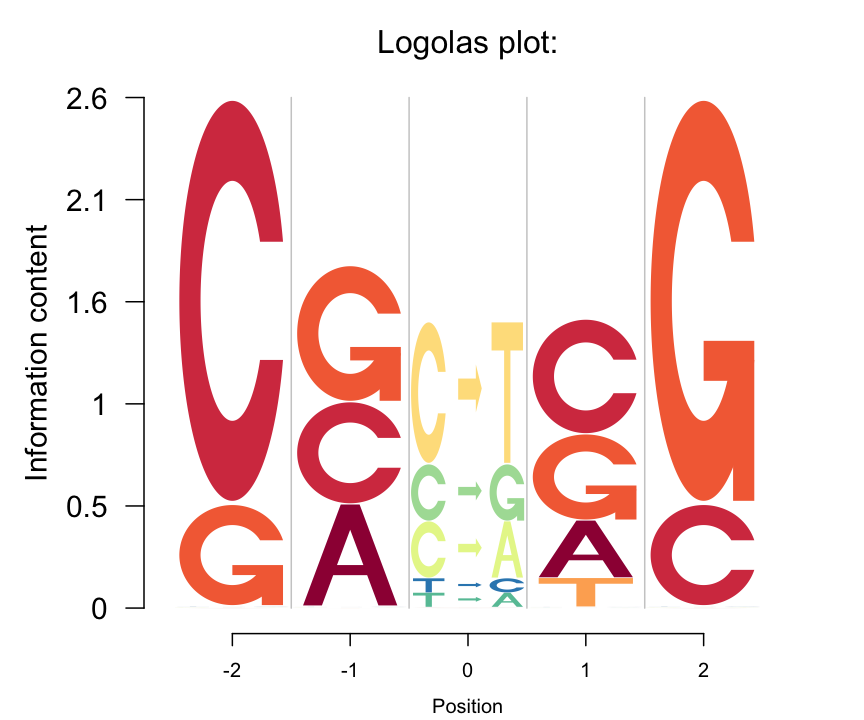
\includegraphics[width=6in,height=5in]{figure/logolas_use_7_0-1} 

\end{knitrout}
\end{center}
\end{figure}

One issue with this plot is that the user may want to have the C in \begin{verb} C>T \end{verb}
to be of the same color, but here the symbol C and \begin{verb} C>T \end{verb} are treated
as separate entities. However Logolas coloring profile provides the user the flexibility to color each symbol instead of a string. We use the color type \begin{verb} per_symbol \end{verb} instead of the \begin{verb} per_row \end{verb} profile we have been using so far.

\begin{figure}[htp]
\begin{center}
\begin{knitrout}
\definecolor{shadecolor}{rgb}{0.969, 0.969, 0.969}\color{fgcolor}\begin{kframe}
\begin{alltt}
\hlstd{cols} \hlkwb{=} \hlstd{RColorBrewer}\hlopt{::}\hlstd{brewer.pal.info[RColorBrewer}\hlopt{::}\hlstd{brewer.pal.info}\hlopt{$}\hlstd{category} \hlopt{==} \hlstr{'qual'}\hlstd{,]}
\hlstd{col_vector} \hlkwb{=} \hlkwd{unlist}\hlstd{(}\hlkwd{mapply}\hlstd{(RColorBrewer}\hlopt{::}\hlstd{brewer.pal, cols}\hlopt{$}\hlstd{maxcolors,} \hlkwd{rownames}\hlstd{(cols)))}

\hlstd{total_chars} \hlkwb{=} \hlkwd{c}\hlstd{(}\hlstr{"A"}\hlstd{,} \hlstr{"B"}\hlstd{,} \hlstr{"C"}\hlstd{,} \hlstr{"D"}\hlstd{,} \hlstr{"E"}\hlstd{,} \hlstr{"F"}\hlstd{,} \hlstr{"G"}\hlstd{,} \hlstr{"H"}\hlstd{,} \hlstr{"I"}\hlstd{,} \hlstr{"J"}\hlstd{,} \hlstr{"K"}\hlstd{,} \hlstr{"L"}\hlstd{,} \hlstr{"M"}\hlstd{,} \hlstr{"N"}\hlstd{,} \hlstr{"O"}\hlstd{,}
            \hlstr{"P"}\hlstd{,} \hlstr{"Q"}\hlstd{,} \hlstr{"R"}\hlstd{,} \hlstr{"S"}\hlstd{,} \hlstr{"T"}\hlstd{,} \hlstr{"U"}\hlstd{,} \hlstr{"V"}\hlstd{,} \hlstr{"W"}\hlstd{,} \hlstr{"X"}\hlstd{,} \hlstr{"Y"}\hlstd{,} \hlstr{"Z"}\hlstd{,} \hlstr{"zero"}\hlstd{,} \hlstr{"one"}\hlstd{,} \hlstr{"two"}\hlstd{,}
            \hlstr{"three"}\hlstd{,} \hlstr{"four"}\hlstd{,} \hlstr{"five"}\hlstd{,} \hlstr{"six"}\hlstd{,} \hlstr{"seven"}\hlstd{,} \hlstr{"eight"}\hlstd{,} \hlstr{"nine"}\hlstd{,} \hlstr{"dot"}\hlstd{,} \hlstr{"comma"}\hlstd{,}
            \hlstr{"dash"}\hlstd{,} \hlstr{"colon"}\hlstd{,} \hlstr{"semicolon"}\hlstd{,} \hlstr{"leftarrow"}\hlstd{,} \hlstr{"rightarrow"}\hlstd{)}

\hlkwd{set.seed}\hlstd{(}\hlnum{20}\hlstd{)}
\hlstd{color_profile} \hlkwb{<-} \hlkwd{list}\hlstd{(}\hlstr{"type"} \hlstd{=} \hlstr{"per_symbol"}\hlstd{,}
                      \hlstr{"col"} \hlstd{=} \hlkwd{sample}\hlstd{(col_vector,} \hlkwd{length}\hlstd{(total_chars),} \hlkwc{replace}\hlstd{=}\hlnum{FALSE}\hlstd{))}

\hlkwd{logomaker}\hlstd{(table,}
          \hlkwc{color_profile} \hlstd{= color_profile,}
          \hlkwc{total_chars} \hlstd{= total_chars,}
          \hlkwc{frame_width} \hlstd{=} \hlnum{1}\hlstd{,}
          \hlkwc{ic.scale} \hlstd{=} \hlnum{TRUE}\hlstd{,}
          \hlkwc{yscale_change}\hlstd{=}\hlnum{TRUE}\hlstd{,}
          \hlkwc{xlab} \hlstd{=} \hlstr{"Position"}\hlstd{,}
          \hlkwc{ylab} \hlstd{=} \hlstr{"Information content"}\hlstd{)}
\end{alltt}
\end{kframe}
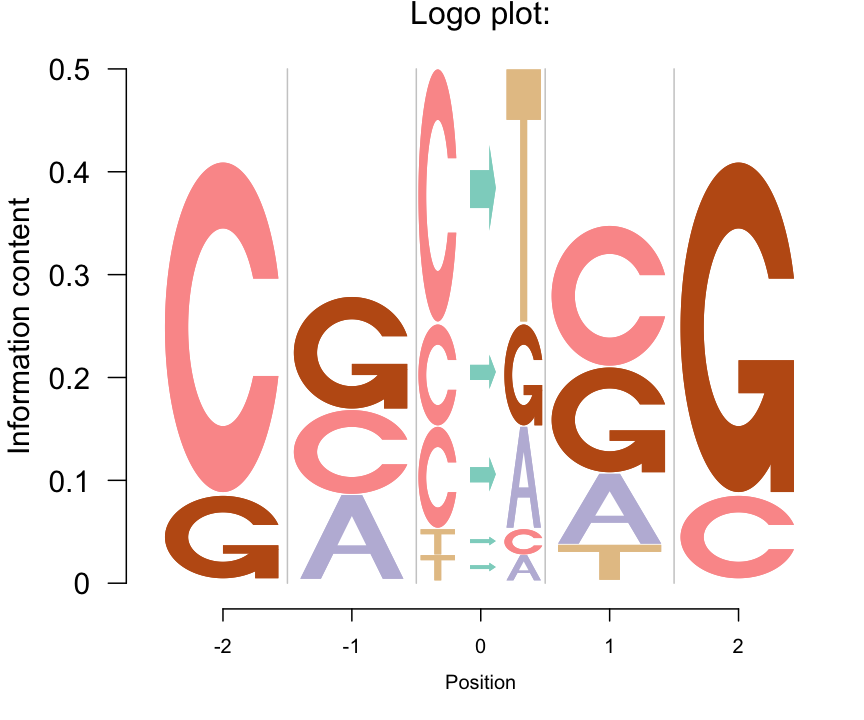
\includegraphics[width=6in,height=5in]{figure/logolas_use_7-1} 

\end{knitrout}
\end{center}
\end{figure}

Another coloring option is \begin{verb} per_column \end{verb}, in which we have a specific color for a specific column.

\clearpage

\subsection{String Logos:  Histone marks patterns}

In studies related to histone marks, one might be interested to see if certain histone marks are prominent than others in some cell lines or tissues or in some genomic regions. In this case, we apply \Logolas{} on an example data from Koch et al (2007) [Supp Table 2 of that paper]. The authors recorded number of histone modification sites identified by their algorithm which overlap with an intergenic sequence, intron, exon, gene start and gene end for the lymphoblastoid cell line, GM06990, in the ChIP-CHIP data. Logolas provides a handy visualization to see how the patterns of histone modification sites changes across genomic region types for that cell line.

First we input the data from Supp Table 2 due to Koch et al (2007).

\begin{knitrout}
\definecolor{shadecolor}{rgb}{0.969, 0.969, 0.969}\color{fgcolor}\begin{kframe}
\begin{alltt}
\hlstd{mat} \hlkwb{<-} \hlkwd{rbind}\hlstd{(}\hlkwd{c}\hlstd{(}\hlnum{326}\hlstd{,} \hlnum{296}\hlstd{,} \hlnum{81}\hlstd{,} \hlnum{245}\hlstd{,} \hlnum{71}\hlstd{),}
             \hlkwd{c}\hlstd{(}\hlnum{258}\hlstd{,} \hlnum{228}\hlstd{,} \hlnum{55}\hlstd{,} \hlnum{273}\hlstd{,} \hlnum{90}\hlstd{),}
             \hlkwd{c}\hlstd{(}\hlnum{145}\hlstd{,} \hlnum{121}\hlstd{,} \hlnum{29}\hlstd{,} \hlnum{253}\hlstd{,} \hlnum{85}\hlstd{),}
             \hlkwd{c}\hlstd{(}\hlnum{60}\hlstd{,} \hlnum{52}\hlstd{,} \hlnum{23}\hlstd{,} \hlnum{180}\hlstd{,} \hlnum{53}\hlstd{),}
             \hlkwd{c}\hlstd{(}\hlnum{150}\hlstd{,} \hlnum{191}\hlstd{,} \hlnum{63}\hlstd{,} \hlnum{178}\hlstd{,} \hlnum{63}\hlstd{))}

\hlkwd{rownames}\hlstd{(mat)} \hlkwb{<-} \hlkwd{c}\hlstd{(}\hlstr{"H3K4ME1"}\hlstd{,} \hlstr{"H3K4ME2"}\hlstd{,} \hlstr{"H3K4ME3"}\hlstd{,} \hlstr{"H3AC"}\hlstd{,} \hlstr{"H4AC"}\hlstd{)}
\hlkwd{colnames}\hlstd{(mat)} \hlkwb{<-} \hlkwd{c}\hlstd{(}\hlstr{"Intergenic"}\hlstd{,}\hlstr{"Intron"}\hlstd{,}\hlstr{"Exon \textbackslash{}n 1000 KB window"}\hlstd{,}
                   \hlstr{"Gene start \textbackslash{}n 1000 KB window"}\hlstd{,}\hlstr{"Gene end \textbackslash{}n 1000 KB window"}\hlstd{)}
\end{alltt}
\end{kframe}
\end{knitrout}

Note here that the histone mark symbols are alphanumeric, for example $H3K4ME1$.
We now apply \Logolas{} on this data.

\begin{figure}[h]
\begin{center}
\begin{knitrout}
\definecolor{shadecolor}{rgb}{0.969, 0.969, 0.969}\color{fgcolor}\begin{kframe}
\begin{alltt}
\hlstd{color_profile} \hlkwb{<-} \hlkwd{list}\hlstd{(}\hlstr{"type"} \hlstd{=} \hlstr{"per_row"}\hlstd{,}
                      \hlstr{"col"} \hlstd{=} \hlkwd{sample}\hlstd{(RColorBrewer}\hlopt{::}\hlkwd{brewer.pal}\hlstd{(}\hlnum{10}\hlstd{,}\hlkwc{name} \hlstd{=} \hlstr{"Spectral"}\hlstd{),}
                          \hlkwd{dim}\hlstd{(mat)[}\hlnum{1}\hlstd{]))}


\hlkwd{logomaker}\hlstd{(mat,}
          \hlkwc{color_profile} \hlstd{= color_profile,}
          \hlkwc{frame_width} \hlstd{=} \hlnum{1}\hlstd{,}
          \hlkwc{ic.scale} \hlstd{=} \hlnum{TRUE}\hlstd{,}
          \hlkwc{pop_name} \hlstd{=} \hlstr{"Histone marks in various genomic regions"}\hlstd{,}
          \hlkwc{xlab} \hlstd{=} \hlstr{""}\hlstd{,}
          \hlkwc{ylab} \hlstd{=} \hlstr{"Information content"}\hlstd{,}
          \hlkwc{yscale_change} \hlstd{=} \hlnum{TRUE}\hlstd{,}
          \hlkwc{col_line_split} \hlstd{=} \hlstr{"black"}\hlstd{)}
\end{alltt}
\end{kframe}
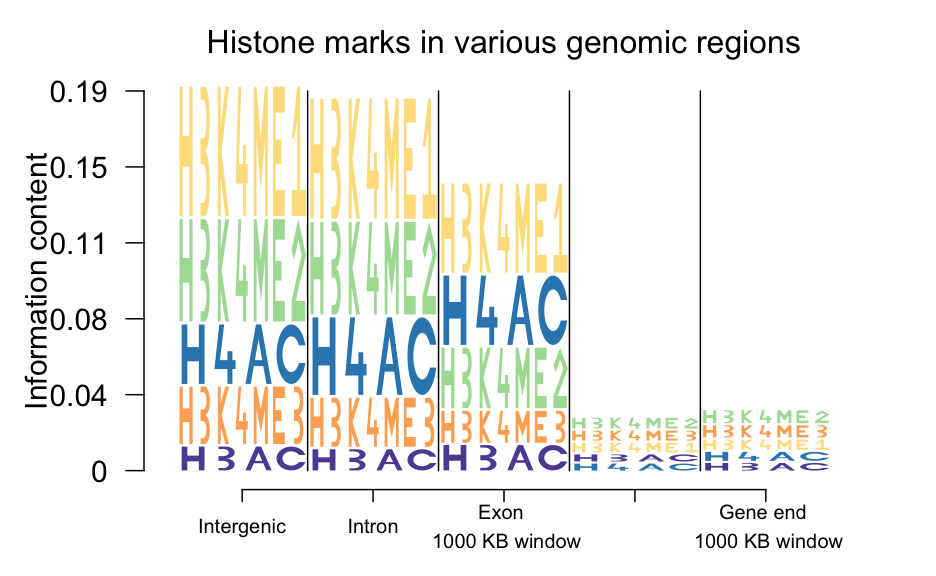
\includegraphics[width=6.5in,height=4in]{figure/histone_logolas-1} 

\end{knitrout}
\end{center}
\end{figure}

\newpage

The \textit{EDLogo} representation of the same table i presented below.

\begin{figure}[h]
\begin{center}
\begin{knitrout}
\definecolor{shadecolor}{rgb}{0.969, 0.969, 0.969}\color{fgcolor}\begin{kframe}
\begin{alltt}
\hlstd{color_profile} \hlkwb{<-} \hlkwd{list}\hlstd{(}\hlstr{"type"} \hlstd{=} \hlstr{"per_row"}\hlstd{,}
                      \hlstr{"col"} \hlstd{=} \hlkwd{sample}\hlstd{(RColorBrewer}\hlopt{::}\hlkwd{brewer.pal}\hlstd{(}\hlnum{10}\hlstd{,}\hlkwc{name} \hlstd{=} \hlstr{"Spectral"}\hlstd{),}
                          \hlkwd{dim}\hlstd{(mat)[}\hlnum{1}\hlstd{]))}

\hlkwd{nlogomaker}\hlstd{(mat,}
          \hlkwc{color_profile} \hlstd{= color_profile,}
          \hlkwc{logoheight} \hlstd{=} \hlstr{"log"}\hlstd{,}
          \hlkwc{pop_name} \hlstd{=} \hlstr{"Histone marks in various genomic regions"}\hlstd{,}
          \hlkwc{xlab} \hlstd{=} \hlstr{""}\hlstd{,}
          \hlkwc{ylab} \hlstd{=} \hlstr{"Information content"}\hlstd{,}
          \hlkwc{yscale_change} \hlstd{=} \hlnum{TRUE}\hlstd{,}
          \hlkwc{col_line_split} \hlstd{=} \hlstr{"black"}\hlstd{)}
\end{alltt}
\end{kframe}
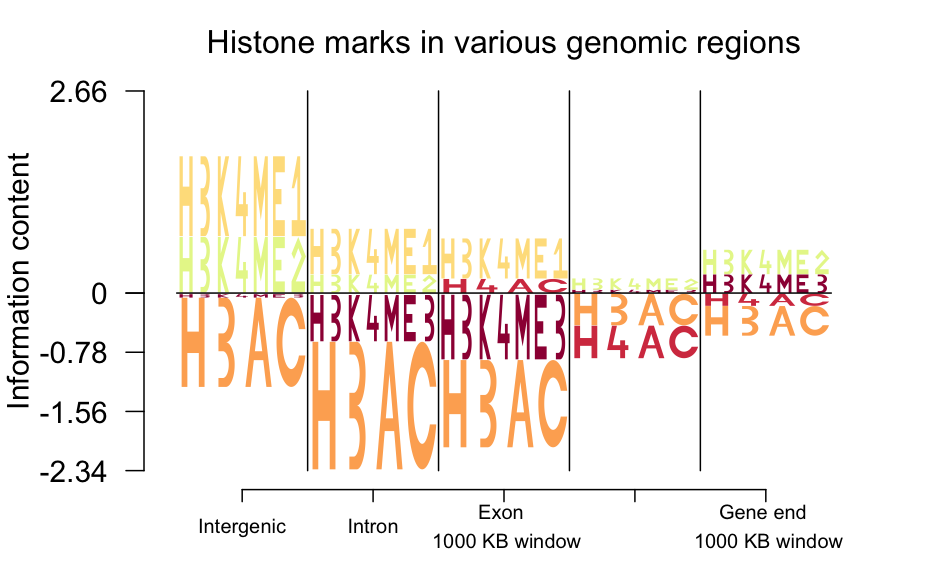
\includegraphics[width=6.5in,height=4in]{figure/histone_nlogolas-1} 

\end{knitrout}
\end{center}
\end{figure}

\newpage


\section{Creating logos and adding to Library}

An user can create her own logo and add to her personalized library and \Logolas{} provides a very simple interface for doing so.

For example, if one wants to have the symbol Lambda as part of her logo,
she can create it as follows

\begin{knitrout}
\definecolor{shadecolor}{rgb}{0.969, 0.969, 0.969}\color{fgcolor}\begin{kframe}
\begin{alltt}
\hlstd{LAMBDAletter} \hlkwb{<-} \hlkwa{function}\hlstd{(}\hlkwc{plot}\hlstd{=}\hlnum{FALSE}\hlstd{,}
                         \hlkwc{fill_symbol} \hlstd{=} \hlnum{TRUE}\hlstd{,}
                         \hlkwc{colfill}\hlstd{=}\hlstr{"green"}\hlstd{,}
                         \hlkwc{lwd}\hlstd{=}\hlnum{10}\hlstd{)\{}

  \hlstd{x} \hlkwb{<-} \hlkwd{c}\hlstd{(}\hlnum{0.15}\hlstd{,} \hlnum{0.5}\hlstd{,} \hlnum{0.85}\hlstd{,} \hlnum{0.75}\hlstd{,} \hlnum{0.5}\hlstd{,} \hlnum{0.25}\hlstd{)}
  \hlstd{y} \hlkwb{<-} \hlkwd{c}\hlstd{(}\hlnum{0}\hlstd{,} \hlnum{1}\hlstd{,} \hlnum{0}\hlstd{,} \hlnum{0}\hlstd{,} \hlnum{0.8}\hlstd{,} \hlnum{0}\hlstd{)}
  \hlstd{fill} \hlkwb{<-} \hlstd{colfill}
  \hlstd{id} \hlkwb{<-} \hlkwd{rep}\hlstd{(}\hlnum{1}\hlstd{,} \hlkwd{length}\hlstd{(x))}

  \hlstd{colfill} \hlkwb{<-} \hlkwd{rep}\hlstd{(colfill,} \hlkwd{length}\hlstd{(}\hlkwd{unique}\hlstd{(id)))}

  \hlkwa{if}\hlstd{(plot)\{}
    \hlkwd{get_plot}\hlstd{(x, y, id, fill, colfill,} \hlkwc{lwd} \hlstd{= lwd,} \hlkwc{fill_symbol} \hlstd{= fill_symbol)}
  \hlstd{\}}

  \hlstd{ll} \hlkwb{<-} \hlkwd{list}\hlstd{(}\hlstr{"x"}\hlstd{= x,}
             \hlstr{"y"}\hlstd{= y,}
             \hlstr{"id"} \hlstd{= id,}
             \hlstr{"fill"} \hlstd{= fill,}
             \hlstr{"colfill"} \hlstd{= colfill)}
  \hlkwd{return}\hlstd{(ll)}
\hlstd{\}}
\end{alltt}
\end{kframe}
\end{knitrout}

One can take a look at the symbol created in the following way.

\begin{knitrout}
\definecolor{shadecolor}{rgb}{0.969, 0.969, 0.969}\color{fgcolor}\begin{kframe}
\begin{alltt}
\hlstd{lambda} \hlkwb{<-} \hlkwd{LAMBDAletter}\hlstd{(}\hlkwc{plot}\hlstd{=}\hlnum{TRUE}\hlstd{)}
\end{alltt}
\end{kframe}

\includegraphics[width=4in,height=4in]{figure/new_symbol-1} 
\begin{kframe}\begin{alltt}
\hlstd{grid}\hlopt{::}\hlkwd{grid.newpage}\hlstd{()}
\hlstd{grid}\hlopt{::}\hlkwd{pushViewport}\hlstd{(grid}\hlopt{::}\hlkwd{viewport}\hlstd{(}\hlkwc{x}\hlstd{=}\hlnum{0.5}\hlstd{,}\hlkwc{y}\hlstd{=}\hlnum{0.5}\hlstd{,}\hlkwc{width}\hlstd{=}\hlnum{1}\hlstd{,} \hlkwc{height}\hlstd{=}\hlnum{1}\hlstd{,}
                                  \hlkwc{clip}\hlstd{=}\hlnum{TRUE}\hlstd{))}
\hlstd{grid}\hlopt{::}\hlkwd{grid.polygon}\hlstd{(lambda}\hlopt{$}\hlstd{x, lambda}\hlopt{$}\hlstd{y,}
                   \hlkwc{default.unit}\hlstd{=}\hlstr{"native"}\hlstd{,}
                   \hlkwc{id}\hlstd{=lambda}\hlopt{$}\hlstd{id,}
                   \hlkwc{gp}\hlstd{=grid}\hlopt{::}\hlkwd{gpar}\hlstd{(}\hlkwc{fill}\hlstd{=lambda}\hlopt{$}\hlstd{fill,}
                                 \hlkwc{lwd}\hlstd{=}\hlnum{10}\hlstd{))}
\end{alltt}
\end{kframe}

\includegraphics[width=4in,height=4in]{figure/new_symbol-2} 

\end{knitrout}

The function name has to be of the form `*letter"` where the user can be creative with the `"*"` part. Also the name must be in uppercase letters. The user can then add this symbol to the logo plot library and make logos of strings containing the above symbol.

\begin{figure}
\begin{center}
\begin{knitrout}
\definecolor{shadecolor}{rgb}{0.969, 0.969, 0.969}\color{fgcolor}\begin{kframe}
\begin{alltt}
\hlstd{counts_mat} \hlkwb{<-} \hlkwd{rbind}\hlstd{(}\hlkwd{c}\hlstd{(}\hlnum{0}\hlstd{,} \hlnum{10}\hlstd{,} \hlnum{100}\hlstd{,} \hlnum{60}\hlstd{,} \hlnum{20}\hlstd{),}
                    \hlkwd{c}\hlstd{(}\hlnum{40}\hlstd{,} \hlnum{30}\hlstd{,} \hlnum{30}\hlstd{,} \hlnum{35}\hlstd{,} \hlnum{20}\hlstd{),}
                    \hlkwd{c}\hlstd{(}\hlnum{100}\hlstd{,} \hlnum{0}\hlstd{,} \hlnum{15}\hlstd{,} \hlnum{25}\hlstd{,} \hlnum{75}\hlstd{),}
                    \hlkwd{c}\hlstd{(}\hlnum{10}\hlstd{,} \hlnum{30}\hlstd{,} \hlnum{20}\hlstd{,} \hlnum{50}\hlstd{,} \hlnum{70}\hlstd{)}
\hlstd{)}
\hlkwd{colnames}\hlstd{(counts_mat)} \hlkwb{<-} \hlkwd{c}\hlstd{(}\hlstr{"Pos 1"}\hlstd{,} \hlstr{"Pos 2"}\hlstd{,} \hlstr{"Pos 3"}\hlstd{,} \hlstr{"Pos 4"}\hlstd{,} \hlstr{"Pos 5"}\hlstd{)}
\hlkwd{rownames}\hlstd{(counts_mat)} \hlkwb{<-} \hlkwd{c}\hlstd{(}\hlstr{"R/LMBD/Q"}\hlstd{,} \hlstr{"A"}\hlstd{,} \hlstr{"X"}\hlstd{,} \hlstr{"Y"}\hlstd{)}

\hlstd{color_profile} \hlkwb{<-} \hlkwd{list}\hlstd{(}\hlstr{"type"} \hlstd{=} \hlstr{"per_row"}\hlstd{,}
                      \hlstr{"col"} \hlstd{= RColorBrewer}\hlopt{::}\hlkwd{brewer.pal}\hlstd{(}\hlkwd{dim}\hlstd{(counts_mat)[}\hlnum{1}\hlstd{],} \hlkwc{name} \hlstd{=} \hlstr{"Spectral"}\hlstd{))}
\hlkwd{logomaker}\hlstd{(counts_mat,}
          \hlkwc{color_profile} \hlstd{= color_profile,}
          \hlkwc{frame_width} \hlstd{=} \hlnum{1}\hlstd{,}
          \hlkwc{addlogos}\hlstd{=}\hlstr{"LMBD"}\hlstd{,}
          \hlkwc{addlogos_text}\hlstd{=}\hlstr{"LAMBDA"}\hlstd{)}
\end{alltt}
\end{kframe}
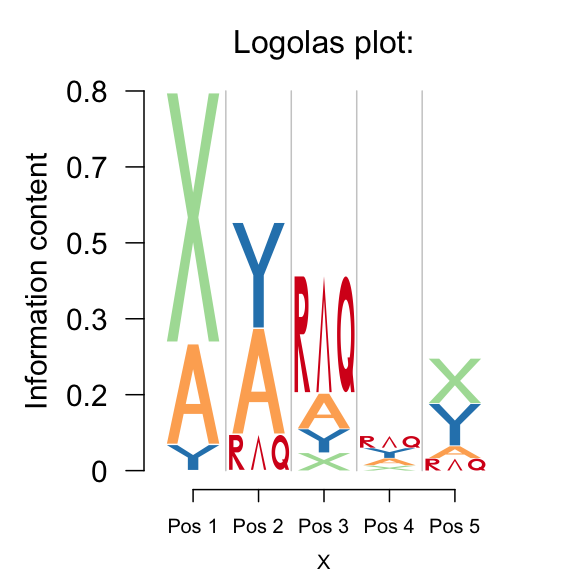
\includegraphics[width=4in,height=4in]{figure/new_string-1} 

\end{knitrout}
\end{center}
\end{figure}


\section{Conclusion}

\Logolas{} provides a new logo representation called \textit{EDLogo} that highlights both enrichment as well as depletion of symbols in a logo plot. It also allows the user to plot strings as logos, that extends the applicability of logo plots beyond DNA, RNA and protein sequences. We show a few examples of the string logo in modeling mutational signature profiles, histone marks composition and ecological species abundance compositions. \Logolas{} also provides an adaptive scaling algorithm called Dirichlet adaptive shrinkage (dash) which scales the position weights for each position adapitvely taking into account the scales of the frequency of alignment at that position. In addition to the aforementioned features, \Logolas{} also provides many novel customizations, fill and border styles, comptability of logo plots with ggplot2 graphics etc.

\section{Acknowledgements}

The authors would like to acknowledge Oliver Bembom, the author of `seqLogo` for acting as an inspiration and providing the foundation on which this package is created. We would also like to thank John Blischak, Kevin Luo, Hussein al Asadi and Alex White for helpful discussions.

\section{Session Info}

\begin{knitrout}
\definecolor{shadecolor}{rgb}{0.969, 0.969, 0.969}\color{fgcolor}\begin{kframe}
\begin{alltt}
\hlkwd{sessionInfo}\hlstd{()}
\end{alltt}
\begin{verbatim}
## R version 3.3.3 (2017-03-06)
## Platform: x86_64-apple-darwin13.4.0 (64-bit)
## Running under: macOS Sierra 10.12.5
## 
## locale:
## [1] en_US.UTF-8/en_US.UTF-8/en_US.UTF-8/C/en_US.UTF-8/en_US.UTF-8
## 
## attached base packages:
## [1] grid      stats     graphics  grDevices utils     datasets  methods  
## [8] base     
## 
## other attached packages:
## [1] ggplot2_2.2.1  gridExtra_2.3  gridBase_0.4-7 Logolas_1.2.1  knitr_1.17    
## 
## loaded via a namespace (and not attached):
##  [1] Rcpp_0.12.12       plyr_1.8.4         gtable_0.2.0       stats4_3.3.3      
##  [5] magrittr_1.5       evaluate_0.10.1    scales_0.4.1       highr_0.6         
##  [9] rlang_0.1.1.9000   stringi_1.1.5      lazyeval_0.2.0     labeling_0.3      
## [13] BiocStyle_2.2.1    RColorBrewer_1.1-2 tools_3.3.3        stringr_1.2.0     
## [17] munsell_0.4.3      seqLogo_1.40.0     colorspace_1.3-2   SQUAREM_2017.10-1 
## [21] tibble_1.3.4
\end{verbatim}
\end{kframe}
\end{knitrout}

\begin{thebibliography}{1}

\bibitem{Bembom2016}
Bembom O (2016).
\newblock seqLogo: Sequence logos for DNA sequence alignments.
\newblock R package version 1.40.0.

\bibitem{Wagih2014}
Omar Wagih (2014).
\newblock RWebLogo: plotting custom sequence logos.
\newblock R package version 1.0.3. https://CRAN.R-project.org/package=RWebLogo

\bibitem{Ou2015}
Jianhong Ou and Lihua Julie Zhu  (2015).
\newblock  motifStack: Plot stacked logos for single or multiple DNA, RNA and amino acid sequence.
\newblock  R package version 1.14.0.

\bibitem{Shiraishi2015}
Shiraishi Y, Tremmel G, Miyano S, Stephens M (2015)
\newblock A Simple Model-Based Approach to Inferring and Visualizing Cancer Mutation Signatures.
\newblock PLoS Genet 11(12): e1005657. doi: 10.1371/journal.pgen.1005657

\bibitem{Koch2007}
Koch CM, Andrews RM, Flicek P, et al (2007).
\newblock The landscape of histone modifications across $1 \%$ of the human genome in five human cell lines.
\newblock Genome Research. 2007;17(6):691-707. doi:10.1101/gr.5704207.

\end{thebibliography}

\end{document}
